\documentclass[oneside]{nccuthesis}
\usepackage{times}
\usepackage{verbatim}
\usepackage{color}
\usepackage{url}
\usepackage{graphicx}
\usepackage{array}
\usepackage{pdfpages} % include outside .pdf
\usepackage{wallpaper} % watermark
% for table generate
\usepackage{mathtools}
\usepackage{amsmath}
\usepackage{amssymb}
\usepackage{booktabs}
\usepackage{adjustbox}
\usepackage{longtable}

% Format the refs
%\usepackage[sort,comma,square ]{natbib}
\usepackage[hidelinks]{hyperref}
% For the tree
\usepackage{tikz}
\usepackage{tikz-qtree}

%Bibliography style
\bibliographystyle{acm}

% For barchart
\usepackage{pgfplots}

% Using the tex-text mapping for ligatures etc.
\defaultfontfeatures{Mapping=tex-text}

% Set the default fonts
\setmainfont{Times New Roman}
\setCJKmainfont{AR PL UKai TW}
\setCJKmonofont{AR PL UKai TW}

% Your information goes here
% author: Tz-Huan Huang [http://www.csie.ntu.edu.tw/~tzhuan]

% ----------------------------------------------------------------------------
% "THE CHOCOLATE-WARE LICENSE":
% Tz-Huan Huang wrote this file. As long as you retain this notice you
% can do whatever you want with this stuff. If we meet some day, and you think
% this stuff is worth it, you can buy me a chocolate in return Tz-Huan Huang
% ----------------------------------------------------------------------------

% Syntax: \var{English}{Chinese}
\university{National Chengchi University (NCCU)}{國立政治大學}
\college{College of Science}{理學院}
\institute{Department of Computer Science}{資訊科學系}
\title{Portfolio Management System with Risk Preference Adjusted Utility Function}
{具風險偏好調整效用函數之資產配置系統}
\author{Tain-Tzu Chang}{張天慈}
\studentid{108971001}
\advisor{Yuh Jong Hu, Ph.D.}{胡毓忠\ 博士}
\defenseyear{2021}{一一零}
\defensemonth{July}{七}
\defenseday{17}

\pgfplotsset{compat=1.14}
\begin{document}

% 政大論文浮水印

\begin{abstracten}
Requirements for portfolio management is different among different investors. Risk is one of the critical factors. Max Drawdown (MDD), the maximum observed loss from a peak to a trough of a portfolio, is a commonly used risk indicator. Reinforcement Learning (RL) is a promising machine learning approach for portfolio selection. Instead of using investment return as a reward function directly, many models use indicators that have taken variability into account, like Sharpe Ratio \cite{Sharpe49} or Sterling ratio. However, neither Sharpe ratio nor Sterling ratio has inputs to raise or reduce risk's influence upon the reward function. Therefore the model using Sharpe Ratio \cite{Sharpe49} or Sterling ratio cannot reflect the needs of investor types with different tolerance to risk.

\par
In this thesis, we introduce a reward function for Portfolio Management RL model which includes the influence of MDD as its parameters.   

asset allocation reinforcement learning reward function


\noindent
Keywords: Reinforcement Learning, Max Drawdown, Portfolio Management,
\end{abstracten}

\input{src/with-watermark.tex}

\hypersetup{pageanchor=false}

\frontmatter
\pagenumbering{gobble}
\makecover

\clearpages
\setcounter{page}{1}
\hypersetup{pageanchor=true}
\pagenumbering{roman}
\phantomsection
\ClearWallPaper
% generate certification
% \makecertification
% or include scanned pdf
\addcontentsline{toc}{chapter}{口試委員會審定書}
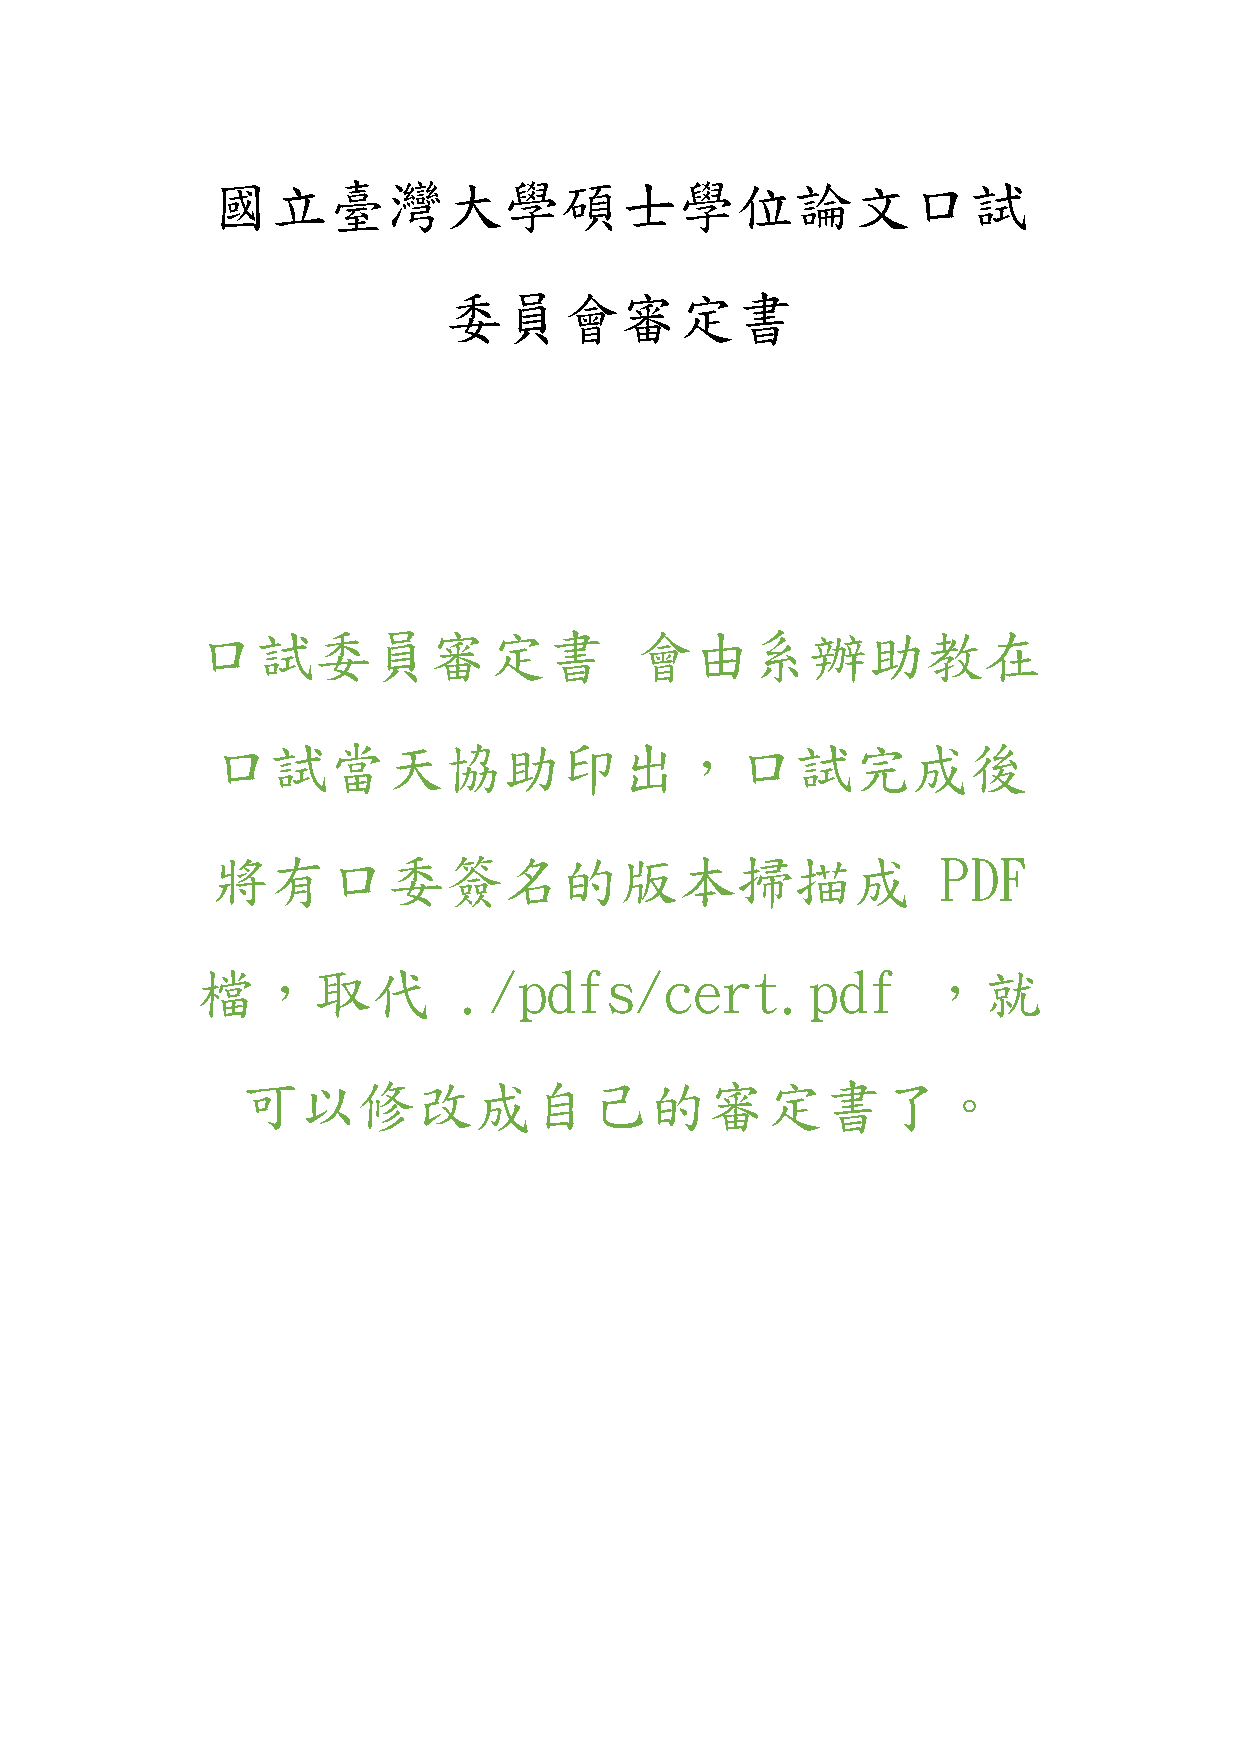
\includepdf[pages={1}]{pdfs/cert.pdf}


%\begin{acknowledgementszh}
這是中文行距測試,應該看到一點五倍行距。這是中文行距測試,應該看到一點
五倍行距。這是中文行距測試,應該看到一點五倍行距。這是中文行距測試,應
該看到一點五倍行距。這是中文行距測試,應該看到一點五倍行距。這是中文行
距測試,應該看到一點五倍行距。這是中文行距測試,應該看到一點五倍行距。
這是中文行距測試,應該看到一點五倍行距。這是中文行距測試,應該看到一點
五倍行距。這是中文行距測試,應該看到一點五倍行距。這是中文行距測試,應
該看到一點五倍行距。這是中文行距測試,應該看到一點五倍行距。這是中文行
距測試,應該看到一點五倍行距。這是中文行距測試,應該看到一點五倍行距。

感謝\ldots
\end{acknowledgementszh}

\begin{acknowledgementsen}


I'm glad to thank\ldots 
\end{acknowledgementsen}

\begin{abstracten}
Requirements for portfolio management is different among different investors. Risk is one of the critical factors. Max Drawdown (MDD), the maximum observed loss from a peak to a trough of a portfolio, is a commonly used risk indicator. Reinforcement Learning (RL) is a promising machine learning approach for portfolio selection. Instead of using investment return as a reward function directly, many models use indicators that have taken variability into account, like Sharpe Ratio \cite{Sharpe49} or Sterling ratio. However, neither Sharpe ratio nor Sterling ratio has inputs to raise or reduce risk's influence upon the reward function. Therefore the model using Sharpe Ratio \cite{Sharpe49} or Sterling ratio cannot reflect the needs of investor types with different tolerance to risk.

\par
In this thesis, we introduce a reward function for Portfolio Management RL model which includes the influence of MDD as its parameters.   

asset allocation reinforcement learning reward function


\noindent
Keywords: Reinforcement Learning, Max Drawdown, Portfolio Management,
\end{abstracten}


% Table of Content
\clearpages
\tableofcontents
% List of Figures
\clearpages
\listoffigures
% List of Tables
\clearpages
\listoftables

\mainmatter

% Your thesis goes here
\chapter{Introduction}
\section {Background}
A portfolio is a collection of financial investments. The goal of portfolio selection is to construct an optimal portfolio, which is usually different between investors due to their characteristics. Among these characteristics, risk preference is one of the significant factors. There are many indicators to represent the risk of the portfolio. Maximum Drawdown (MDD),  maximum loss from a peak over a given period, is a commonly used indicator of the risk.

Traditionally portfolio selection can be divided into two stages. Frist stage constructs the belief of future performance of available financial products. The second stage starts from the first stage and produces the choice of portfolio.  Modern Portfolio Theory (MPT) introduced by  Harry Markowitz \cite{10.2307/2975974} focus on the second stage. Machine Learning (ML) or Reinforcement Learning (RL) can complete both stages in a single process and construct portfolios that out-performed the general market.\cite{KRAUSS2017689}
\section {Motivation}
Psychologically, humans favor avoiding losses to acquire equivalent gains. This tendency is called Loss Aversion.\cite{kahneman2000analysis} Kahneman's study suggests losses are twice as powerful as gains.\cite{Tversky1992} With Modern Portfolio Theory (MPT), we can construct a portfolio that produces the maximum expected return from a given variance, an indicator of risk, or vice versa, the minimal variance from a given expected return.\cite{10.2307/2975974} MPT can construct portfolios fits different investors' preference.
Although many portfolio performance measures are risk-adjusted\cite{cogneau2009101,cogneau2009more,cogneau2009more2}, like the Shape ratio\cite{Sharpe49} or the Sterling ratio\cite{magdon2004maximum}, most of them do not incorporate investors' risk preferences. Constructing portfolios based on investors' risk preferences will challenge machine learning models optimizing with these measures.

\section {Research Objective}
This thesis aims to introduce an objective function and incorporate conventional Deep Reinforcement Learning (DRL) models to construct portfolios that fit investors with different risk preferences. The expected Maximum Drawdown (MDD) of the portfolio will represent investors' risk preferences and adjust the portfolio performance measure, which will be the objective function incorporate with DRL models to construct portfolios based on investors' risk preferences.
\label{c:intro}


\chapter{Approach}
\section{Related Works Study}
We will study works about asset allocation systems related to investors' risk preference or reinforcement learning model. The goal is to understand better the requirement, challenges, and opportunities for our portfolio management system.
\section{Implementation}
We will then design and implement our system, including the trading environment with one of the existing commonly used and advanced models for the deep reinforcement learning model. 
\section{Training and Validation}
After implementing the design, we will define the market features as inputs for the system and select investments from the investable universe to build the portfolio. The goal is to choose investments with low correlations between each other; hence their combinations can yield better profits from the same risk level. We will split available data into two parts, the first part used for training and the rest for validation. We will optimize our design based on the training/validation result iteratively.
\section{Conclusions and Extensions}
The final step is to analyze the validation result to identify our design's strengths and weaknesses. Moreover, we will explore some extensions for further improvement in our proposed portfolio management system.
\chapter{Related Work}
\label{c:related}

%\section{First}
%\label{s:related1}

\section{Risk Adjusted Measures of Performance}
There are many portfolio performance measures.\cite{cogneau2009101,cogneau2009more,cogneau2009more2}
Risk-Adjusted measures incorporate risk into the measure of performance for finance investments and reflect investors' nature better than using return along.
We will discuss a few of them over here.
\subsection{Sharpe Ratio}
Sharpe Ratio\cite{Sharpe49} is one of the most well-known risk-adjusted measure. It represent amount of return per unit of variation, or risk.\\
The revision version is defined as
\[ SR = \frac{E(R_a - R_b)}{\sigma_a},
\sigma_a = \sqrt{VAR(R_a-R_b)}\]
where \(R_a\) is the return of the assert, 
\(R_b\) is the risk-free return,
\(E(R_a - R_b)\) is the expected excess return of the assert,
and \(\sigma_a\) is standard deviation of the excess return.
One downside of the Sharpe Ratio is that it penalizes occasional high returns\cite{9206647}.
\subsection{Sterling ratio}
Sterling ratio\cite{magdon2004maximum} uses max drawdown (MDD) over a given period to represent the risk; this resolves the issue Sharpe Ratio has with occasional high returns. 
There are many forms of Sterling ratio; one common definition\cite{magdon2004maximum} is defined as 
\[ SR = \frac{E(R_a - R_b)}{MDD - 10\%}\]
\subsection{Calmar ratio}
Calmar ratio\cite{young1991calmar} replace empirical max drawdown with the expected maximum drawdown \(E(MDD)\), defined as 
\[C_T = \frac{E(R_a - R_b)}{E(MDD)}\]


\subsection{Other Measures of Performance}
There are many other Sharpe ratio variations, like Burke Ratio, Martin Ratio, or Pain Ratio\cite{bacon2009sharp}. Furthermore, Philippe Cogneau and Georges Hübner censused the 101 performance measures for portfolios. Many of the measures are risk-adjusted measures\cite{cogneau2009101,cogneau2009more,cogneau2009more2}.
\section{Modern Portfolio Theory (MPT)}
Harry Markowitz introduced modern portfolio theory (MPT) in 1952. Instead of maximizing the expected return, the objective of MPT is to find the maximum expected return on a given risk. The variance of the portfolio is used as an indicator of risk. \cite{10.2307/2975974}
\par
For an N assets portfolio, \(E(R_i)\) and  \(\sigma_i\) is the expected return and standard deviation of the asset \(i\). \(w_i\) is the weighting of the asset in the portfolio.\(\rho_{ij}\) is the correlation coefficient between the returns on assets i and j.
The expected return and variance of the portfolio, \(E(R_p)\) and \(\sigma_p^2\), are defined as:
\[E(R_p) = \sum_i^N w_i E_i\]
\[\sigma_p^2 = \sum_i \sum_j w_i w_j \sigma_i \sigma_j \rho_{ij}\]
where
\[\forall w: w \geq 0 \quad \sum_i ^N w_i = 1\]
\par
The next step is plot expected return and variance of all portfolios and find the efficient frontier. Than we can identify the portfolio with the maximize return on a given risk, or, vice versa, the lowest risk on a given expected return from the efficient frontier.
\section{Financial Market Predictions with Machine Learning}
Machine Learning has become a powerful tool in many fields, including finance. Christopher Krauss successfully used various machine learning techniques, including deep neural networks, gradient-boosted-trees, and random forests, to create ensembles predicting the S\&P 500 index that out-performed the general market\cite{KRAUSS2017689}.
\par

Thomas Fischer brings deep learning to the next level by using Long Short-Term Memory (LSTM) network\cite{FISCHER2018654}. His model demonstrates LSTM can effectively extract meaningful information from noisy financial time series data and beat other machine learning models in  Christopher Krauss's article  \cite{KRAUSS2017689} for most situations, except the crisis in 2009, where Random Forest perform better than LSTM.
\section{Trading systems with Reinforcement Learning}
John Moody and Lizhong Wu introduced Reinforcement Learning for the trading system \cite{618952}. Trading systems trained via Reinforcement learning can incorporate the effects of transaction costs and taxes. The result of such systems outperformed trading systems trained via supervised learning with labels. For objective function, they observed maximizing the differential Sharpe ratio yields more consistent results than maximizing profits\cite{618952,moody1998performance}.\\
The differential Sharpe ratio \(D\) is defined as:
\[
\cfrac{d D_t}{d R_t} = 
\cfrac{B_{t-1}-A_{t-1} R_t}{(B_{t-1}-A_{t-1}^2)^\frac{3}{2}}
\]
where
A and B is the first and second moments of the returns' distributions
\[ A_n = \cfrac{1}{n}\sum_{i=1}^nR_i\quad
B_n = \cfrac{1}{n}\sum_{i=1}^nR_i^2
\]

Saud Almahdi uses a coherent downside risk measure, the Calmar ratio,  as the objective function for Reinforcement Learning \cite{AdaptivePortfolioTradingSystem}. They show that the portfolios constructed using RRL with the expected maximum drawdown based Calmar ratio results yield better performance and transaction cost resilient than the portfolios constructed with the Sharpe ratio. 






\cite{AdaptivePortfolioTradingSystem}
\section{Soft Actor-Critic (SAC)}
Soft Actor-Critic (SAC)\cite{haarnoja2018soft}


\chapter{Implementation}
\label{c:implement}
\section{Overview}


\begin{figure}[h!]
  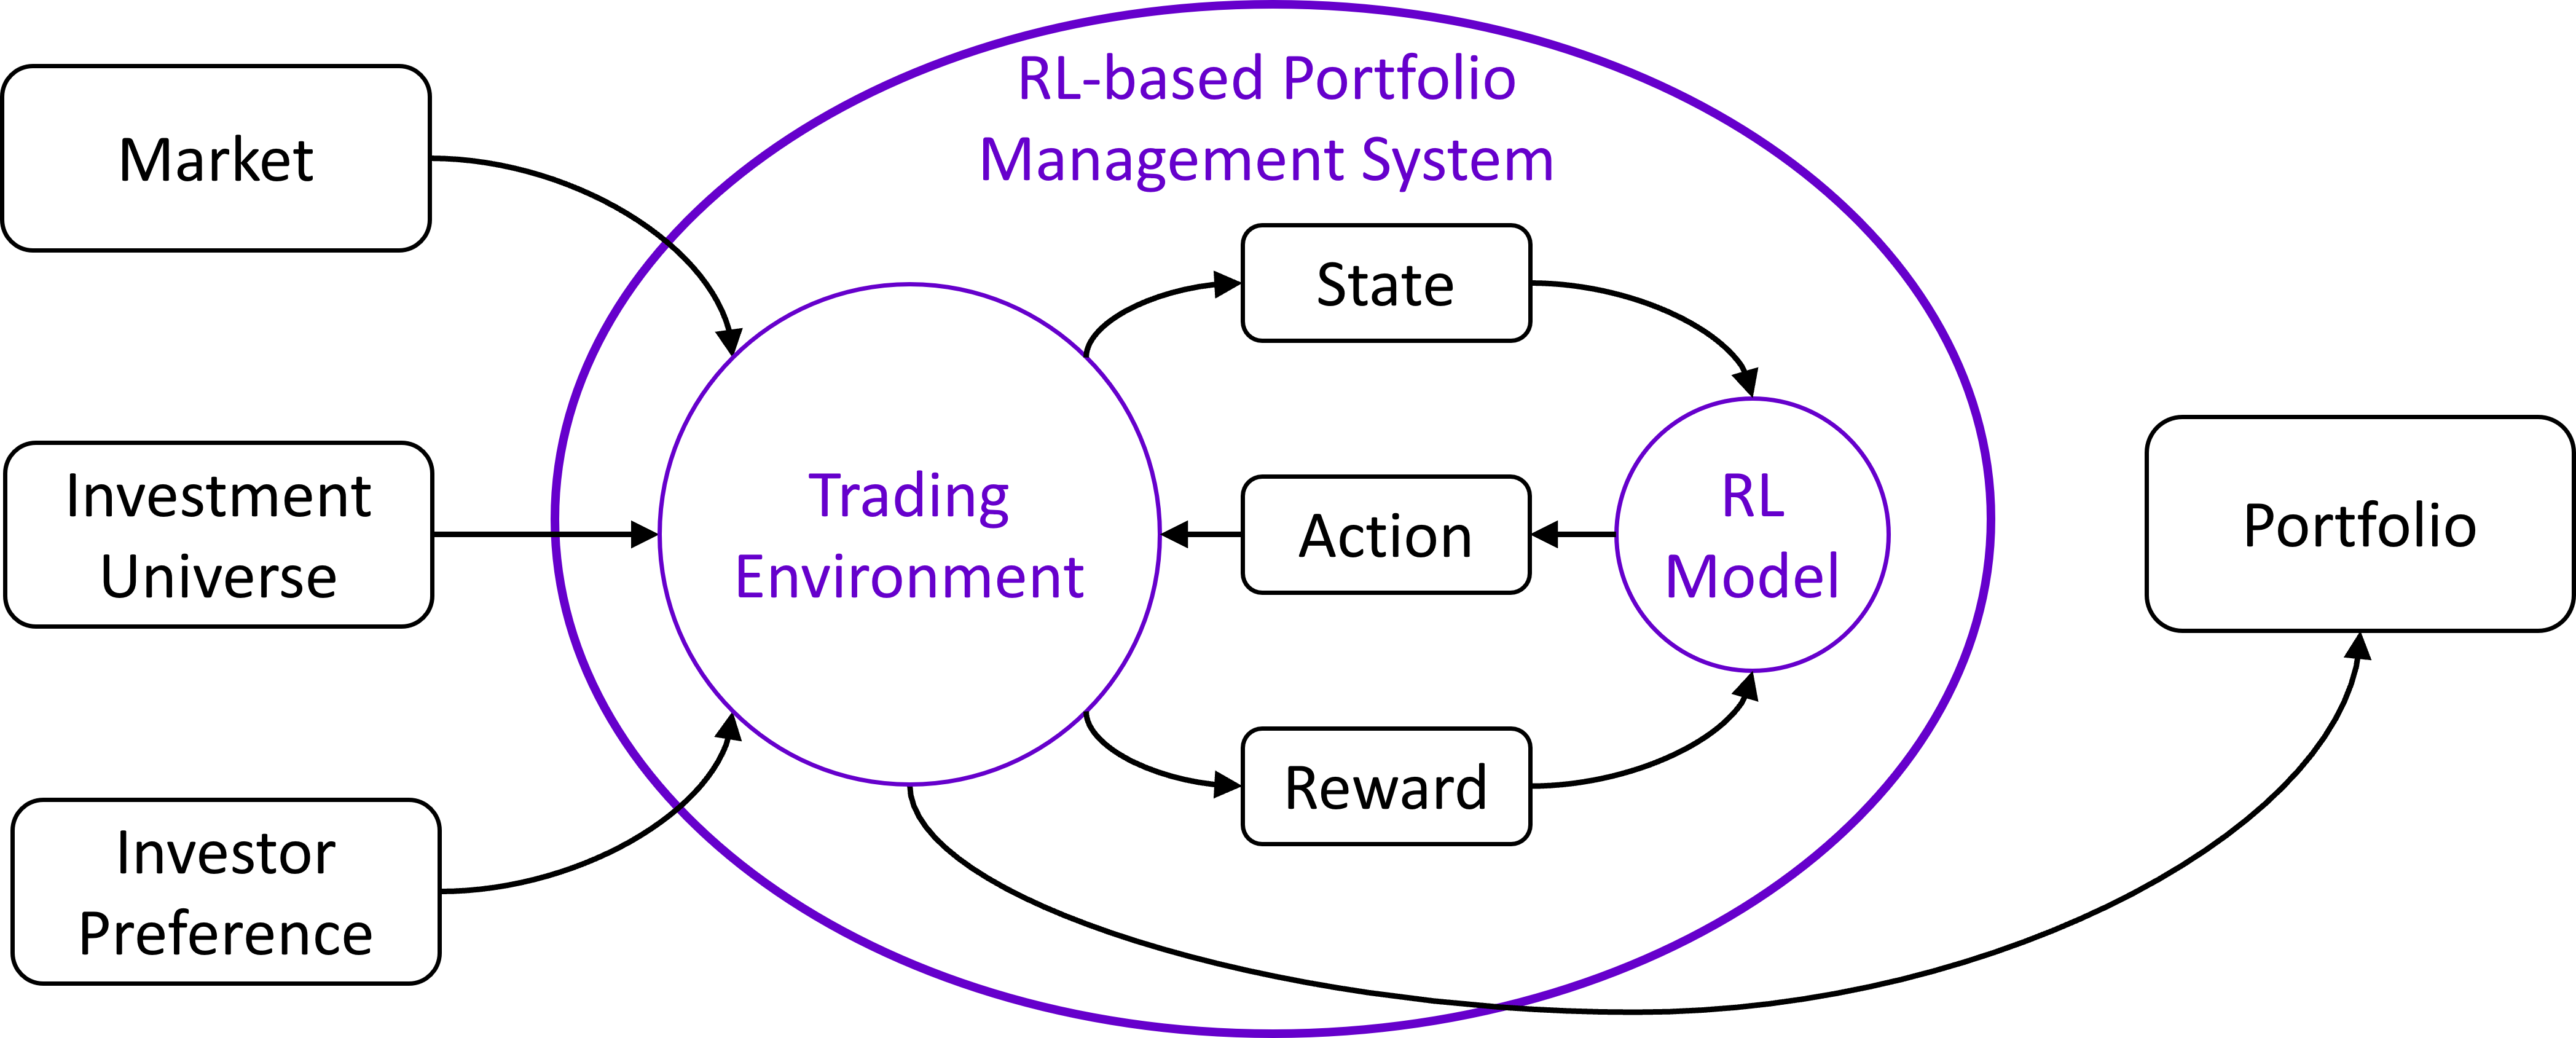
\includegraphics[width=15cm]{images/context_diagram.png}
  \caption{The birds}
  \label{fig:birds}
\end{figure}
\section{Market}
\section{Investments}
Investments are the investable universe for the portfolio management system. The goal is to choose investments with low covariances between each other; hence their combinations can yield better profits from the same risk level. We start from the top 100 ETFs by Asset Under Management (AUM) on March 2021 and remove ones with trading records of less than 14 years. We then obtain the top two most correlated ETFs and remove the one with lower AUM and continue the same process iteratively until 30 ETFs are left.  (\autoref{appendix:etfs})
\par


\section{Investor Preference}
\section{Reinforcement Learning Model}
Soft Actor-Critic (SAC)\cite{haarnoja2018soft}

\appendix
\chapter{Selection of ETFs}
\label{appendix:etfs_corr}
\par
\begin{longtable}{|| m{2cm}| m{11.5cm}||}
\hline
Symbol & Name  \\ \hline \hline
SPY&SPDR S\&P 500 ETF \\ \hline
AGG&iShares Core U.S. Aggregate Bond ETF \\ \hline
BND&Vanguard Total Bond Market ETF \\ \hline
GLD&SPDR Gold Trust \\ \hline
LQD&iShares iBoxx \$ Investment Grade Corporate Bond ETF \\ \hline
BSV&Vanguard Short-Term Bond ETF \\ \hline
MBB&iShares MBS Bond ETF \\ \hline
IGSB&iShares Short-Term Corporate Bond ETF \\ \hline
SHY&iShares 1-3 Year Treasury Bond ETF \\ \hline
SHV&iShares Short Treasury Bond ETF \\ \hline

\end{longtable}
\chapter{Market Features}
\label{appendix:features_list}
\par
\begin{longtable}{|| m{10cm}| m{3.5cm}||}
\hline
Description & Categories \\ \hline \hline
5-Year Treasury Constant Maturity Rate & Interest Rates\\ \hline
10-Year Treasury Constant Maturity Rate & Interest Rates\\ \hline
30-Year Treasury Constant Maturity Rate & Interest Rates\\ \hline
5-Year Breakeven Inflation Rate & Interest Rates\\ \hline
10-Year Breakeven Inflation Rate & Interest Rates\\ \hline
Crude Oil Prices: Brent - Europe &  Commodities\\ \hline
Gold Prices &  Commodities\\ \hline
Dow Jones Industrial Average &  Indexes\\ \hline
NASDAQ Composite Index &  Indexes\\ \hline
CBOE Volatility Index (VIX) &  Indexes\\ \hline
US Dollar Index (USDX) &  Currencies\\ \hline
\end{longtable}



\chapter{Temp}

\section{Measure}
\(DD_T\)\cite{moody2001learning}
\[
DD_T = \sqrt{\cfrac{1}{T}\sum_{t=0}^{T}{min\{R_T,0\}^2}}
\]

VaR (Value at Risk)\cite{CoherentMeasuresofRisk}
\[
VaR_\alpha(X) = -inf \{x |P[X\leq x\cdot r]>\alpha \}
\]
Measure
RISK TOLERANCE FUNCTIONS\cite{elton2009modern}

\[f=\bar{R}-\frac{\tau^2}{T} \]
where T is referred to as risk tolerance and expresses the investor’s trade-off between
expected return and variance of return. 
\par
SAFETY FIRST\cite{elton2009modern}
If \(R_P\) is the return on the portfolio and \(R_L\) is the level below which the investor does not wish returns
to fall, Roy’s criterion is
\[Minimize P(R_p<R_L) \]
\section{Bitcoin}
%\chapter{Conclusions and Extensions}
\label{c:conclusion}
\secton{Conclusions}
\section{Extensions}


\@startappendix


\backmatter

\clearpages
\phantomsection
\addcontentsline{toc}{chapter}{\bibname}
% Your bibliography goes here

\bibliography{
    bib/thesis-finance.bib,
    bib/thesis-ml.bib,
    bib/thesis-misc.bib
}


\end{document}
